% Chapter Template

\chapter{Arbitrage theory in continuous time finance} % Main chapter title

\label{Chapter2} % Change X to a consecutive number; for referencing this chapter elsewhere, use \ref{ChapterX}

%----------------------------------------------------------------------------------------
%	SECTION 1
%----------------------------------------------------------------------------------------

\section{Financial markets}

\begin{figure}[th]
\centering
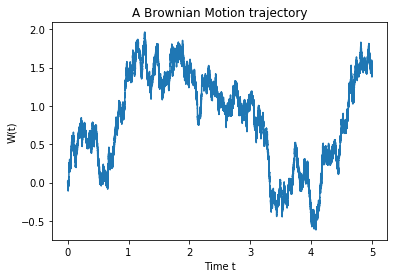
\includegraphics{Figures/brownianMotion.png}
\decoRule
\caption[A Wiener process trajectory]{}
\label{fig:BM}
\end{figure}


In the financial markets there is a lot of players and different types of investments. The classical investments are bonds and stocks, where you either lending or buying equity. The big players are commercial banks, investment banks, insurance companies and pension funds. The derivatives are depending on an underlying asset, where the dependency is specified in the contract. The options discussion in the introduction are all depending on a underlying stock. The contract can be constructed in many ways, hence it gives more options to construct your portfolio (see Appendix \ref{AppendixA} for examples). When pricing financial product we use the market to price derivatives (This correspond to the equivalent martingale measure $\mathbb{Q}$ to the objective measure $\mathbb{P}$), so we do not introduce arbitrage to the market. In the classic Black Scholes formula for European options, we will assume following about the market:
\theoremstyle{assumption}
\begin{assumption}{}\label{EfficientMarket}
We assume following institutional facts:
\begin{enumerate}
\item[•] Short positions and fractional holding are allowed 
\item[•] There are no bid-ask spread, i.e. selling price is equal to buying price
\item[•] There are no transactions costs of trading.
\item[•] The market is completely liquid, i.e. it is possible to buy/sell unlimited quantities on the market. You can borrow unlimited amount from the bank by selling short.
\end{enumerate}
(see p. 6 \parencite{finKont})
\end{assumption}
We can discuss these assumptions at length, but in order to progress mathematically, we need to accept them for now. There is some justification for liquidity on vanilla options, because those options gets traded on large scale. Before going into the mathematics of the Black Scholes formula, we need to introduce key concepts.
%-----------------------------------
%	SUBSECTION 1
%-----------------------------------

\subsection{Financial Derivatives}
There a broad range of different derivatives. In this thesis, we will mainly divide derivatives into two classes. 
\begin{enumerate}
\item Simple derivatives (T-claims)
\item Exotic derivatives
\end{enumerate}
The first class is the simple derivaties or T-claims. These are simple because you can only exercise them at maturity (time T). The exotic derivatives is all kind of functions on the underlying assets, where you have more options than exercise at termination time. There are so many derivatives, hence the list will not be comprehensive at all. Some important simple derivatives will be the European calls and puts, because we can price analytically.

\theoremstyle{definition}
\begin{definition}{European Call Option:}\label{ECall}
A Europeann call option is a option where the owner of the option has the option to exercise at maturity. The contract function for the derivative:
\begin{equation}
\begin{split}
\phi(S(T))=\max\{S(T)-K, 0\}
\end{split}
\end{equation}
Where S(T) is the price of underlying asset at maturity and K is the agreed strike price.
\end{definition}
For illustration of above contract see appendix \ref{AppendixA}.

\parencite{finKont}


%-----------------------------------
%	SUBSECTION 2
%-----------------------------------

\subsection{Self-financing portfolio (Without consumption)}
A self-financing portfolio h, is a portfolio h which doesn't get any external injection of money. h is the number of each assets in our portfolio. We denote $V^{h}(t)$ the value of our portfolio h at time t, hence:
\theoremstyle{definition}
\begin{definition}{Self-financing portfolio}
A portfolio consisting of N+1 assets: \\
h(t)=($h_0(t),h_1(t), \dotsc, h_{N}$) is self-financing if:
\begin{equation}\label{SF}
\begin{split}
dV^{h}(t)=\sum_{i=0}^{N} h_{i}(t) dS_{i}(t)
\end{split}
\end{equation}
Where $S_{i}$ is the $i'th$ asset in our portfolio, N+1 is the total number of assets and\\
$V^{h}(t)=\sum_{i=0}^{N} h_{i}(t) S_{i}(t)$
\end{definition}
The important takeaway is that a S-F portfolio is kind of a budget restriction. You are only allowed to reallocate your assets within the portfolio but not injecting cash into the portfolio. The concept is important for the discussion of arbitrage and hedging.

%-----------------------------------
%	SUBSECTION 3
%-----------------------------------
\subsection{Arbitrage}
Arbitrage is the financial term for a "free lunch". An investor can profit without bearing risk, if there is arbitrage on the market. In order to avoid making a "money machine", we want to price derivatives to be arbitrage free.  
\theoremstyle{definition}
\begin{definition}{Arbitrage:}
An arbitrage possibility on a financial market is a self-financed portfolio h suct that
\begin{equation}\label{Arbitrage}
\begin{split}
V^{h}(0)=0\\
P(V^{h}(T)\geq 0)=1\\
P(V^{h}(T)>0)>1
\end{split}
\end{equation}
We say that the market is arbitrage free if there aro no arbitrage possibilities.\\
(see p. 96 \parencite{finKont})
\end{definition}
From the definition a self-financing portfolio fullfilling equation \eqref{Arbitrage} would give the possiblility for arbitrage. The investor in this portfolio starts with 0 dollars, and without injecting any money, the investor is certain of not losing any money. In addition he has a positive probability by ending up with more than 0 at maturity. Arbitrage is a way to price financial products "fair". To price "fair" and hedge againt risk will be the topics for this thesis.

%-----------------------------------
%	SUBSECTION 4
%-----------------------------------

\subsection{Complete Market and Hedging}
Hedging is a concepts to protect against exposure to risk. A hedge is simply a risk neutralization action in order to minimize the overall risk. In the defition below, we define a hedge for an simply T-claim \eqref{tClaim}.
\theoremstyle{definition}
\begin{definition}{Hedging and completeness for T-claim:}
A T-claim X can be hedged, if there exist a self-financing portfolio h s.t.:
\begin{enumerate}
\item[•] $V^{h}(T)=X$ P-a.s.
\end{enumerate}
I.e. h is an hedge portfolio for X if it is guaranteed to pay in all circumstances an amount identical to the payout of X.\\
The market is complete, if every derivative is hedgable.
(see p. 115 \parencite{finKont})
\end{definition}
Hedging and completeness means the same for other derivatives than T-claims, but for now we will only show the concepts for the T-claim.

%----------------------------------------------------------------------------------------
%	SECTION 2
%----------------------------------------------------------------------------------------

\section{Black-Scholes Formula two dimensionel}
In addition to our assumptions for the financial market, we also assume:\\
\theoremstyle{assumption}
\begin{assumption}{Black-Scholes assumptions}\label{BS-Assumption}
We assume following ideal conditions in addition to \eqref{EfficientMarket}:
\begin{enumerate}
\item[•] The short-term interest rate is known and is constant through time 
\item[•] The stock price follows a Geometric Brownian Motion. The $\sigma$ is constant.\item[•] The stock pays no dividends or other distributions.
\item[•] The option is a simple option ("European" see \eqref{ECall}).
\end{enumerate}
(see p. 640 \parencite{B-S-Paper})
\end{assumption}

We assume the underlying stock follows a geometric brownian motion:
$dS(t)=\alpha S dt + \sigma S dW_t$ where the solution to the SDE is given as
\begin{equation}\label{GBM}
\begin{split}
S(t)=S(0) \cdot \exp \bigg( (\alpha -\frac{1}{2} \sigma^2) t + \sigma W(t) \bigg)
\end{split}
\end{equation}

The $\mu$ and $\sigma$ have clear empirical meanings.


\begin{theorem}\label{BS-PDE}
\textbf{Black-Scholes PDE:}
blabla
\begin{align}
F_t(t,s)+rsF_s(t,s)+\frac{1}{2} s^2 \sigma^2(t,s)F_{ss}(t,s) -rF(t,s)&=0\\
F(T,s)&=\Phi(s)
\end{align}
\end{theorem}
The below proposition is a consequence of the B-S equation:

\theoremstyle{proposition}
\begin{proposition}{}\label{BS-price-EuroCall}
\textbf{Black-Scholes formula for call option:} The price of a European call option with strike K and maturity T is given by the formula  $\Pi(t)=F(t,S(t)$, where
\begin{align*}
F(t,s)=s \cdot N(d_1(t,s)) - e^{-r(T-t)}\cdot K \cdot N(d_2(t,s))
\end{align*}
N is the cumulative distribution function of a standard normal distribution $\mathcal{N}(0,1)$ and
\begin{align*}
d_1(t,s)=\frac{1}{\sigma\cdot \sqrt{T-t}} \cdot \bigg( \ln(\frac{s}{K}) + (r+\frac{1}{w} \sigma^2) (T-t) \bigg)\\
d_2(t,s)=d_1(s,t)-\sigma \sqrt{T-t}
\end{align*}
(see p. 105 \parencite{	finKont})
\end{proposition}


The above formula for the European call option is actually the same for an American call option, but is not true for an American put option or for call options paying dividends. The result for the American call option was shown by Merton \parencite{Merton73}, that the intrinsic value is never greater than the worth of the option given by the risk-neutral valuation formula \parencite{finKont}.



\begin{theorem}\label{RNVF}
\textbf{Risk-neutral valuation formula:} Given Q is the EMM
\begin{align}
\Pi(t, X)= exp(-r(T-t))\cdot E_{t,x}^Q[X]
\end{align}
\end{theorem}


\theoremstyle{proposition}
\begin{proposition}{}\label{Put-call-parity}
\textbf{Put-call parity:} 
Assume the call and put option has same strike price and time to maturity.
\begin{align*}
p(t,s)=K\cdot \exp(-r(T-t))+c(t,s)-s
\end{align*}
(see p. 126 \parencite{finKont})
\end{proposition}


